\section{Ceros de función}

\subsection{Problema}

Dada $f : \mathbb{R} \to \mathbb{R}$, buscamos un $x^* \in \mathbb{R}$ tal que $f(x^*) = 0$. El número $x^*$ se llama cero o raíz de $f$.

En ciertos casos, como por ejemplo para $f(x)$ un polinomio de grado menor o igual que 2, el problema tiene una solución que sabemos calcular en forma exacta. En otros casos, por ejemplo para $f(x) = e^x - \ln(x^2)$, no parece tan claro cómo calcular una raíz, si es que existe una.

\subsection{Propuesta}

Para calcular una raíz, construiremos una sucesión $\{x_n\}_{n \in \mathbb{N}_0}$ de modo tal que $x_n \xrightarrow[n \to \infty]{} x^*$. Más aún, definiremos dicha sucesión en forma recurrente, de modo tal que a partir de $x_0$ podamos computar $x_1$, luego $x_2$ y así sucesivamente. Esto nos da un método iterativo, en el cual a medida que el número de iteraciones $n$ crece, la aproximación $x_n$ de $x^*$ es cada vez mejor, en el sentido de que el valor absoluto $|x_n - x^*|$ es cada vez más pequeño.

Sin saber aún cómo construir $\{x_n\}_n$, surgen algunas preguntas:

\begin{enumerate}
	\item ¿Cuán rápido convergerá $x_n$ a $x^*$? En otras palabras, ¿con qué velocidad la diferencia $|x_n - x^*|$ converge a 0?

	\item ¿Cuánto es necesario iterar para obtener una buena aproximación? Recordemos que la raíz $x^*$, a la que queremos converger, no es conocida de antemano, con lo cual, en general, no sabemos cuán cerca está $x_n$ de $x^*$ en un instante dado de la iteración.
	
	\item Dado que no podemos iterar infinitamente, necesitamos establecer criterios para decidir cuándo finalizar la iteración, que no dependan de la distancia entre $x_n$ y $x^*$.
\end{enumerate}

\subsection{Velocidad u orden de convergencia}

Como hemos planteado, nos interesa medir la velocidad con la que $\{x_n\}_n$ se aproxima a $x^*$.

\begin{defi}
Sea $\{x_n\}_n$ una sucesión que converge a $x^*$, pero $x_n \neq x^*$ para todo $n$. Decimos que $\{x_n\}_n$ tiene orden de convergencia $p > 0$ si

\[\lim\limits_{n \to \infty} \frac{|x_{n + 1} - x^*|}{|x_n - x^*|^p} = c \neq 0\]

para cierta constante $c \in \mathbb{R}$. Si $p = 1$ decimos que la convergencia es lineal.
Si $1 < p < 2$ decimos que la convergencia es supralineal.
Si $p = 2$ decimos que la convergencia es cuadrática.
\end{defi}

Observemos que si el orden de convergencia es $p$ entonces $|x_{n + 1} - x^*|$ es asintóticamente equivalente a $|x_n - x^*|^p$. Esto implica que, asintóticamente, el error absoluto se reduce polinomialmente, con exponente $p$.

Dado que algunas sucesiones convergen con velocidad variable, no siempre es posible aplicar la anterior definición. Hay una medida más general de la velocidad de convergencia, dada por la siguiente

\begin{defi}
Sea $\{\alpha_n\}_n$ convergente a $\alpha$. Sea $\{\beta_n\}_n$ convergente a 0. Decimos que $\{\alpha_n\}_n$ tiene orden de convergencia $\mathcal{O}(\beta_n)$ (o que $\alpha_n$ converge tan rápido como $\beta_n$) si existe una constante $c > 0$ tal que $\left|\alpha_n - \alpha \right| \leq c \beta_n$ para todo $n$ suficientemente grande. 

En este caso, si $\{\beta_n\}_n$ tiene orden de convergencia $p$, decimos que $\{\alpha_n\}_n$ tiene orden de convergencia al menos $p$. 
\end{defi}

\subsubsection{Interpretación}

¿Qué significa que $\{x_n\}_n$ converja a $x^*$ con orden $p$? Llamemos $e_n = x_n - x^*$. Según la definición de antes, esto significa que $\lim\limits_{n \to \infty}{\frac{|e_{n + 1}|}{|e_n|^p}} = c$ para cierta constante $c \neq 0$. Que $c$ no sea infinito, significa que $|e_{n}|^p$ no tiende a 0 más rápido de lo que lo hace $|e_{n + 1}|$. Que $c$ sea no nulo, significa que $|e_{n + 1}|$ tampoco lo hace más rápido que $|e_{n}|^p$. Por lo tanto, $|e_{n + 1}|$ y $|e_{n}|^p$ convergen a 0 con la misma velocidad o, dicho de otro modo, son asintóticamente equivalentes.

A su vez, es posible interpretar el significado de esta velocidad, en términos prácticos. Dada la equivalencia asintótica de $|e_{n + 1}|$ y $|e_n|^p$, vamos a suponer que para $n$ suficientemente grande $|e_{n + 1}| \approx |e_n|^p$. Supongamos que hasta el término $n$-ésimo llevamos calculados $k$ dígitos decimales del valor $x^*$, es decir que $|e_n| \approx 10^{-k}$. Entonces, $|e_{n + 1}| \approx (10^{-k})^p = 10^{-kp}$, es decir que en el $(n + 1)$-ésimo término, la cantidad de decimales calculados se multiplica por $p$.

Entonces, por ejemplo, que una sucesión converja cuadráticamente significa, a nivel práctico, que la cantidad de dígitos decimales calculados se duplica a cada paso.

\subsection{Criterios de parada}
Respondemos a la tercera pregunta que nos hicimos previamente.

\begin{itemize}
	\item Fijar un número máximo $N$ de iteraciones.
	
	\item Fijar $\varepsilon > 0$ y terminar cuando $|x_n - x_{n - 1}| < \varepsilon$. 
	
	Esto es, terminar cuando los saltos de la sucesión sean chicos.
	
	Este criterio puede fallar. Por ejemplo, tomemos $x_n = \sum_{k = 1}^n \frac{1}{k}$ la sucesión de números armónicos. Como $x_n - x_{n - 1} = \frac{1}{n} \xrightarrow[n \to \infty]{} 0$ entonces para cualquier $\varepsilon > 0$ existirá un valor de $n$ suficientemente grande para el cual dos términos sucesivos disten menos de $\varepsilon$. Sin embargo, es bien sabido que los números armónicos divergen.
	
	\item Fijar $\varepsilon > 0 $ y terminar cuando $\frac{|x_n - x_{n - 1}|}{|x_{n - 1}|} < \varepsilon$. 
	
	Esto es, terminar cuando la sucesión no de saltos demasiado grandes en términos relativos.
	
	\item Fijar $\varepsilon > 0$ y terminar cuando $|f(x_n)| < \varepsilon$. 
	
	Este criterio se basa en que si $x_n$ converge a una raíz, entonces cuando la sucesión converja, $f(x_n)$ será pequeño.
	
	También puede fallar. Por ejemplo, en el caso en que $f(x)$ está muy cerca de cero en un punto pero no tiene una raíz en el entorno (e. g. $f(x) = \frac{1}{x}$).
	
	\item Fijar $\varepsilon > 0$ y terminar cuando $|f(x_n) - f(x_{n - 1})| < \varepsilon$.
	
	\item Fijar $\varepsilon > 0$ y terminar cuando $\frac{|f(x_n) - f(x_{n - 1})|}{|f(x_{n - 1})|} < \varepsilon$.
\end{itemize}

Dado que todos estos criterios son heurísticos, pueden fallar. La elección del criterio adecuado dependerá del contexto.

A continuación exploraremos algunas formas de encontrar una tal sucesión $\{x_n\}_n$ que converja a una raíz.

\subsection{Método de Bisección}

Supongamos que tenemos una función $f:[a, b] \to \mathbb{R}$ contínua, a la que le queremos calcular una raíz. Supongamos, además, que $f(a)f(b) < 0$, es decir, $f(a)$ y $f(b)$ tienen signos opuestos. Consideremos el Algoritmo \ref{algo:bisec}, que asume que estamos en estas condiciones.

\begin{algorithm}
\label{algo:bisec}
\dontprintsemicolon

%\SetKwInOut{Input}{input}
%\SetKwInOut{Output}{output}

%\Input{}
%\Output{}

Sean $a_0 = a$, $b_0 = b$\;
\For{$k = 1$ \KwTo $N$}{
	$c_{k - 1} = \frac{a_{k - 1} + b_{k - 1}}{2}$\;
	Si $f(c_{k - 1})$ cumple con el criterio de parada, terminar\;
	Si $f(c_{k - 1})f(a_{k - 1}) < 0$, entonces $a_k = a_{k - 1}$, $b_k = c_{k - 1}$\;
	Si $f(c_{k - 1})f(b_{k - 1}) < 0$, entonces $a_k = c_{k - 1}$, $b_k = b_{k - 1}$\;
}

\caption[]{Método de Bisección}
\end{algorithm}

El algoritmo determina tres sucesiones $\{a_n\}_n$, $\{b_n\}_n$ y $\{c_n\}_n$. En cada paso elige a $c_n$ como el punto medio entre $a_n$ y $b_n$. 

\begin{obs}
Las lineas 5 y 6 garantizan que

\begin{itemize}
\item $a_n \leq c_n \leq b_n$ para todo $n$.

\item $f(a_n)f(b_n) < 0$ para todo $n$.

\item La sucesión $\{a_n\}_n$ es creciente, mientras que $\{b_n\}_n$ es decreciente.
\end{itemize}
\end{obs}

Veamos que la sucesión $\{c_n\}_n$ converge a una raíz de $f$.

\begin{lema}
\label{lema:sucs}
\[b_n - a_n \leq \frac{b_0 - a_0}{2^n}\]

\begin{proof}
Por inducción en $n \in \mathbb{N}_0$.

Si $n = 0$, no hay nada que ver.

Sea $n > 0$. Es fácil ver que las lineas 5 y 6 del algoritmo eligen $a_n$ y $b_n$ de modo tal que $b_n - a_n \leq \frac{b_{n - 1} - a_{n - 1}}{2}$. Por hipótesis inductiva, $b_{n - 1} - a_{n - 1} \leq \frac{b_0 - a_0}{2^{n - 1}}$ y usando la desigualdad anterior llegamos al resultado buscado.
\end{proof}
\end{lema}

En particular, esto muestra que $\lim\limits_{n \to \infty}(b_n - a_n) = 0$.

\begin{propo}
La sucesion $\{c_n\}_n$ es convergente. Más aún $\lim\limits_{n \to \infty} c_n$ es una raíz de $f$.

\begin{proof}
Como $a_n \leq b_n$ para todo $n$, y $\{b_n\}_n$ es decreciente, entonces $\{a_n\}_n$ está acotada superiormente, por ejemplo por $b_0$. Además $\{a_n\}_n$ es creciente. Luego, es una sucesión convergente. Sea $\ell = \lim\limits_{n \to \infty} a_n$.

Análogamente, $\{b_n\}_n$ es una sucesión decreciente acotada inferiormente, por ejemplo por $a_0$, con lo cual es convergente. Luego $0 = \lim\limits_{n \to \infty} (b_n - a_n) = \lim\limits_{n \to \infty} b_n - \ell$, con lo cual $\lim\limits_{n \to \infty} b_n = \ell$.

Como $a_n \leq c_n \leq b_n$, entonces $\{c_n\}_n$ está acotada entre dos sucesiones que convergen al mismo límite. Por Sandwich, debe ser $\lim\limits_{n \to \infty} c_n = \ell$. En definitiva, $\{a_n\}_n$, $\{b_n\}_n$ y $\{c_n\}_n$ convergen las tres y tienen el mismo límite.

Falta ver que $f(\ell) = 0$. Si fuera $f(\ell) > 0$ entonces, como $f$ es contínua y $a_n$ tiende a $\ell$, tendríamos $f(a_n) > 0$ para todo $n$ suficientemente grande. Análogamente, $f(b_n) > 0$ para todo $n$ suficientemente grande. Pero esto contradice el hecho de que $f(a_n)f(b_n) < 0$ para todo $n$. Análogamente, no puede ser $f(\ell) < 0$. Entonces no queda otra que $f(\ell) = 0$.

\end{proof}
\end{propo}

Esto demuestra que el método siempre converge a una raíz de la función. En lo que sigue llamaremos $x^* = \lim\limits_{n \to \infty} c_n$.

\begin{obs}
De la monotonía de las sucesiones se deduce que $a_n \leq x^* \leq b_n$ para todo $n$.
\end{obs}

\begin{propo}
\[|c_n - x^*| \leq \frac{b_0 - a_0}{2^{n + 1}}\]

\begin{proof}
Como $a_n \leq x^* \leq b_n$ y $c_n$ es el punto medio, entonces $|c_n - x^*| \leq \frac{b_n - a_n}{2}$. Por el Lema \ref{lema:sucs}, se deduce $|c_n - x^*| \leq \frac{b_0 - a_0}{2^{n + 1}}$.
\end{proof}
\end{propo}

\begin{coro}
El orden de convergencia de $\{c_n\}_n$ es al menos lineal.

\begin{proof}
Se desprende de que $\frac{b_0 - a_0}{2^{n + 1}}$ converge linealmente.
\end{proof}
\end{coro}

\subsubsection{Ventajas y desventajas}

\paragraph{Ventajas}

\begin{itemize}
	\item Para cada $a_n$ y $b_n$, nos alcanza con conocer el signo de $f(a_n)$ y el de $f(b_n)$ con lo cual podría no ser necesario evaluar la función $f$ en esos puntos. Esto es conveniente en contextos en los cuales la evaluación es una operación costosa y es posible conocer el signo por alguna vía sencilla.
	\item Tenemos una cota para el error absoluto.
	\item Es fácil encontrar puntos iniciales $a_0$ y $b_0$ factibles.
\end{itemize}

\paragraph{Desventajas}

\begin{itemize}
	\item Asegura una convergencia de orden al menos lineal, aunque puede resultar lenta.
\end{itemize}

\subsection{Problemas de punto fijo}

\begin{defi}
Sea $g: [a, b] \to \mathbb{R}$. Un punto $p \in [a, b]$ se llama punto fijo de $g$ si $g(p) = p$.
\end{defi}

Un problema de cálculo de raíces de una función $f(x)$ puede ser transformado en un problema de punto fijo. Por ejemplo si $g(x) = x + f(x)$ entonces $p$ es raíz de $f$ si y solo si $p$ es punto fijo de $g$.

La conveniencia de transformar el problema de cálculo de una raíz en un problema de punto fijo, se debe a que se conocen varios métodos para resolver esto último, como veremos a continuación.

\begin{propo}
Sea $g:[a, b] \to [a, b]$ contínua. Entonces $g$ tiene punto fijo en $[a, b]$. Si además es derivable y $|g'(x)| < 1$ para todo $x \in (a, b)$, entonces el punto fijo es único.

\begin{proof}
Primero veamos que $g$ tiene un punto fijo en $[a, b]$. Notemos que como $a \leq g(x) \leq b$, entonces $g(a) \geq a$ y $g(b) \leq b$. Si $g(a) = a$, listo. Si no, $g(a) > a$. Análogamente, si $g(b) = b$, terminamos. Si no, $g(b) < b$. Tenemos, entonces, $g(a) - a > 0$ y $g(b) - b < 0$.

Consideremos $f(x) = g(x) - x$. Por lo anterior, $f(a) > 0$ y $f(b) < 0$. Además $f$ es contínua en $[a, b]$ pues $g$ lo es. Luego, por Teorema de Bolzano, existe $p \in (a, b)$ tal que $f(p) = 0$, es decir que $g(p) - p = 0$ o bien $g(p) = p$, con lo cual $p$ es un punto fijo de $g$.

Veamos la unicidad. Sean $p_1, p_2 \in [a, b]$ puntos fijos de $g$, entonces $g(p_1) = p_1$ y $g(p_2) = p_2$. Como $g$ es derivable, por el Teorema del Valor Medio tenemos que

\[|g(p_1) - g(p_2)| = \left|p_1 - p_2\right| \left|g'(\xi)\right|\]

para cierto $\xi$ entre $p_1$ y $p_2$. Pero $|g(p_1) - g(p_2)| = |p_1 - p_2|$, entonces

\[|p_1 - p_2| = \left|p_1 - p_2\right| \left|g'(\xi)\right|\]

Por hipótesis, $\left|g'(\xi)\right| < 1$, con lo cual no queda otra que $|p_1 - p_2| = 0$, i. e., $p_1 = p_2$.

\end{proof}
\end{propo}

Dadas estas condiciones de existencia y unicidad de punto fijo, construimos una sucesión convergente a un punto fijo.

\begin{propo}
\label{propo:ptofijo}
Sea $g:[a, b] \to [a, b]$ contínua y derivable, tal que existe una constante no negativa $k$ tal que $|g'(x)| \leq k < 1$ para todo $x \in (a, b)$. Sea $\{x_n\}_n$ una sucesión tal que 

%\[x_0 \in [a, b] \text{ y } x_{n + 1} = g(x_n) \text{ si }n \geq 0\] 
\[x_0 \in [a, b]\]
\[x_{n + 1} = g(x_n) \text{ si }n \geq 0\] 

Entonces $\{x_n\}_n$ converge al único punto fijo de $g$.

\begin{proof}
Por la Proposición anterior, $g$ posee un único punto fijo en $[a, b]$, que llamamos $p$. Observemos que como $g(x) \in [a, b]$ y $x_0 \in [a, b]$, entonces todo término de la sucesión cae en $[a, b]$.

Queremos ver que $\lim \limits_{n \to \infty} x_n = p$. Notemos que si $n > 0$,

\[|x_n - p| = |g(x_{n - 1}) - g(p)|\]

Como $g$ es derivable, por el Teorema del Valor Medio existe $\xi_{n - 1}$ entre $x_{n - 1}$ y $p$, tal que

\[|g(x_{n - 1}) - g(p)| = \left|x_{n - 1} - p\right| \left|g'(\xi_{n - 1})\right|\]

Como $\left|g'(\xi_{n - 1})\right| \leq k$ entonces

\[|g(x_{n - 1}) - g(p)| \leq \left|x_{n - 1} - p\right| k\]

Por la primera de las igualdades, concluimos que

\[|x_n - p| \leq \left|x_{n - 1} - p\right| k\]

Inductivamente, es fácil ver que

\[|x_n - p| \leq \left|x_0 - p\right| k^n\]

Como $0 \leq k < 1$, $\left|x_0 - p\right| k^n$ tiende a 0 a medida que $n \to \infty$. Por el Teorema del Sandwich, $\lim \limits_{n \to \infty} |x_n - p| = 0$, con lo cual $\lim \limits_{n \to \infty} x_n = p$.

\end{proof}
\end{propo}

Esta técnica para encontrar el punto fijo se llama \textit{iteración de punto fijo}. Bajo ciertas condiciones podemos asegurar el orden de convergencia de la sucesión.

\begin{propo}
\label{propo:conv}
Sea $g \in C^{r}([a, b])$ tal que $p \in (a, b)$ es punto fijo y

\[g'(p) = g''(p) = \cdots = g^{(r - 1)}(p) = 0\text{, } g^{(r)}(p) \neq 0\]

Entonces, si $x_{n + 1} = g(x_n)$ converge a $p$, su orden de convergencia es $r$.

\begin{proof}
Como $g \in C^r([a, b])$, consideramos el desarrollo de Taylor de $g$ de orden $r - 1$, centrado en $p$,

\[g(x) = g(p) + g'(p) (x - p) + \cdots + \frac{g^{(r - 1)}(p)}{(r - 1)!} (x - p)^{r - 1} + \frac{g^{(r)}(\xi_x)}{r!} (x - p)^r = g(p) + \frac{g^{(r)}(\xi_x)}{r!} (x - p)^r\]

con $\xi_x$ entre $x$ y $p$. Evaluando en $x_n$ obtenemos

\[g(x_n) = g(p) + \frac{g^{(r)}(\xi_n)}{r!} (x_n - p)^r\]

con $\xi_n$ entre $x_n$ y $p$. Como $g(x_n) = x_{n + 1}$ y $g(p) = p$,

\[x_{n + 1} - p = \frac{g^{(r)}(p)}{r!} (x_n - p)^r\]

o sea que

\[\frac{x_{n + 1} - p}{(x_n - p)^r} = \frac{g^{(r)}(p)}{r!}\]

Tomando límite en ambos miembros,

\[\lim\limits_{n \to \infty} \frac{x_{n + 1} - p}{(x_n - p)^r} = \frac{g^{(r)}(p)}{r!}\]

Como esta expresión converge, su módulo también lo hace, y

\[\lim\limits_{n \to \infty} \frac{|x_{n + 1} - p|}{|x_n - p|^r} = \frac{|g^{(r)}(p)|}{r!}\]

Como $g^{(r)}(p) \neq 0$ entonces el límite $\frac{|g^{(r)}(p)|}{r!}$ es no nulo. Luego, el orden de convergencia de $\{x_n\}_n$ es $r$.

\end{proof}
\end{propo}

%\subsection{Interpretación de la velocidad de convergencia}

\subsection{Método de Newton}

Supongamos que dada una $f: \mathbb{R} \to \mathbb{R}$, queremos hallar una raíz. Para esto queremos encontrar una función $g: \mathbb{R} \to \mathbb{R}$, cuya expresión involucre a $f$, de modo tal que los puntos fijos de $g$ sean raíces de $f$. Más aún, vamos a pedir que la iteración de punto fijo asociada a $g$ converja cuadráticamente.

Proponemos $g(x) = x - h(x)f(x)$ siendo $h$ una función que todavía no conocemos. Notemos que si $p$ es punto fijo de $g$ entonces $p = g(p) = p - h(p)f(p)$, con lo cual si $h(p) \neq 0$ resulta que $f(p) = 0$. Por lo tanto, todo punto fijo de $g$ es una raíz de $f$, sea cual sea la función $h$ tal que $h(p) \neq 0$.

Como queremos un orden de convergencia cuadrático, pedimos que $g'(p) = 0$. Como $g'(x) = 1 - h'(x)f(x) - h(x) f'(x)$, entonces

\begin{align*}
g'(p) = 0 &\Leftrightarrow 1 - h'(p)f(p) - h(p)f'(p) = 0\\
&\Leftrightarrow 1 - h(p)f'(p) = 0\\
&\Leftrightarrow h(p) = \frac{1}{f'(p)}
\end{align*}

suponiendo que $f'(p) \neq 0$. Entonces podemos tomar $h(x) = \frac{1}{f'(x)}$, que cumple $h(p) \neq 0$. Así, queda

\[g(x) = x - \frac{f(x)}{f'(x)}\]

con lo cual la iteración de punto fijo asociada es

\[x_{n + 1} = g(x_n) = x_n - \frac{f(x_n)}{f'(x_n)}\]

En lo que sigue vamos a ver que esta sucesión efectivamente converge a un punto fijo de $g$ (bajo ciertas condiciones), y lo hace cuadráticamente.

\begin{propo}
Sea $f \in C^2([a, b])$. Sea $p \in (a, b)$ tal que $f(p) = 0$, $f'(p) \neq 0$. Entonces existe $\delta > 0$ tal que toda sucesión $\{x_n\}_n$ con

%\[x_0 \in [p - \delta, p + \delta] \text{ y } x_{n + 1} = x_n - \frac{f(x_n)}{f'(x_n)} \text{ si } n \geq 0\]
\[x_0 \in [p - \delta, p + \delta]\]
\[x_{n + 1} = x_n - \frac{f(x_n)}{f'(x_n)} \text{ si } n \geq 0\]

está bien definida y converge.

\begin{proof}
Sea $g(x) = x - \frac{f(x)}{f'(x)}$.

\begin{itemize}
\item \textbf{$g$ está bien definida en un entorno de $p$.} Como $f'$ es contínua en $[a, b]$ y $p \in (a, b)$ entonces $f'$ es contínua en $p$. En particular, existe $\delta_1 > 0$ tal que $f'(x) \neq 0$ para todo $x \in [p - \delta_1, p + \delta_1]$.

\item \textbf{$g$ es estable en un entorno de $p$.} Notemos que $g'(x) = \frac{f(x)f''(x)}{f'(x)^2}$, que está bien definida en $[p - \delta_1, p + \delta_1]$.

Como $g'(p) = 0$ y $g'$ es contínua en $p$, entonces existe $\delta_2 > 0$, $\delta_2 \leq \delta_1$ tal que, para alguna constante $k$, $|g'(x)| \leq k < 1$ para todo $x \in (p - \delta_2, p + \delta_2)$.
 
Luego, si $x \in [p - \delta_2, p + \delta_2]$, utilizando el Teorema del Valor Medio, deducimos que

\[|g(x) - g(p)| = \left|g'(\xi_x)\right| \left| x - p \right|\]

para $\xi_x$ entre $x$ y $p$. Entonces $|g'(\xi_x)| < 1$. Como además $g(p) = p$ resulta que

\[|g(x) - p| < |x - p| \leq \delta_2\]

Luego $|g(x) - p| \leq \delta_2$, es decir que $g(x) \in [p - \delta_2, p + \delta_2]$.

\end{itemize}

Por lo tanto, $g: [p - \delta_2, p + \delta_2] \to [p - \delta_2, p + \delta_2]$ está bien definida y además $|g'(x)| \leq k < 1$ para todo $x \in (p - \delta_2, p + \delta_2)$. Poniendo $\delta = \delta_2$, una sucesión $\{x_n\}_n$ tal que $x_0 \in [p - \delta, p + \delta]$ y $x_{n + 1} = g(x_n) = x_n - \frac{f(x_n)}{f'(x_n)}$ está en las condiciones de la Proposición \ref{propo:ptofijo}, con lo cual converge a un punto fijo de $g$.

\end{proof}
\end{propo}

Observemos que este resultado sólo asegura la convergencia cuando comenzamos la iteración dentro de un entorno suficientemente chico del punto fijo. En general, no conocemos la localización del punto fijo así como tampoco cuán chico debe ser el entorno. Por esta razón, se suele partir desde un punto arbitrario, e iterar, revisando si se logra converger. En caso negativo, se elige otro punto de partida y se repite la iteración.

Otra forma de sortear el problema es aplicar, inicialmente, algunas iteraciones del método de Bisección y cuando el entorno que contiene a la raíz es suficientemente chico, proceder con Newton.

\begin{propo}
Sea $f \in C^2$ y $p \in \mathbb{R}$ una raíz de $f$. Sea $\{x_n\}_n$ la iteración de punto fijo dada por $x_{n + 1} = x_n - \frac{f(x_n)}{f'(x_n)}$. Supongamos que está bien definida y que nunca vale $p$. Si $e_n = x_n - p$, entonces

\[\frac{e_{n + 1}}{e_n^2} = \frac{1}{2} \frac{f''(\xi_n)}{f'(x_n)}\]

con $\xi_n$ un valor entre $x_n$ y $p$. Más aún, si $f'(p), f''(p) \neq 0$ y la iteración converge a $p$, entonces lo hace con orden cuadrático.

\begin{proof}

Para cada $n \in \mathbb{N}_0$, consideremos el desarrollo de Taylor de $f$ de orden 1 centrado en $x_n$,

\[f(x) = f(x_n) + f'(x_n) (x - x_n) + \frac{f''(\xi_n)}{2} (x - x_n)^2\]

con $\xi_n$ entre $x_n$ y $x$. Evaluando en $p$ obtenemos

\[f(p) = f(x_n) + f'(x_n) (p - x_n) + \frac{f''(\xi_n)}{2} (p - x_n)^2\]

con $\xi_n$ entre $x_n$ y $p$. Luego,

\[0 = f(x_n) - f'(x_n) e_n + \frac{f''(\xi_n)}{2} e_n^2\]

Con un poco de aritmética llegamos a la ecuación buscada,

\[\frac{e_{n + 1}}{e_n^2} = \frac{1}{2} \frac{f''(\xi_n)}{f'(x_n)}\]

Resta ver que si $f'(p) \neq 0$ y $\{x_n\}_n$ converge a $p$, entonces lo hace cuadráticamente. Para esto, debemos ver que $\frac{|e_{n + 1}|}{|e_n|^2}$ converge a una constante no nula. Tomando módulo en la ecuación anterior,

\[\frac{|e_{n + 1}|}{|e_n|^2} = \frac{1}{2} \frac{|f''(\xi_n)|}{|f'(x_n)|}\]

Como $f'$ es contínua, y $\lim\limits_{n \to \infty} x_n = p$, entonces

\[\lim\limits_{n \to \infty} f'(x_n) = f'(p) \neq 0\]

Por otro lado, como $\xi_n$ siempre cae entre $x_n$ y $p$, y $f''$ es contínua, resulta que

\[\lim\limits_{n \to \infty} f''(\xi_n) = f''(p)\]

Por lo tanto, estas dos últimas expresiones convergen en módulo y, más aún,

\[\lim\limits_{n \to \infty} \frac{|e_{n + 1}|}{|e_n|^2} = \lim\limits_{n \to \infty} \frac{1}{2}\frac{|f''(\xi_n)|}{|f'(x_n)|} = \frac{1}{2}\frac{|f''(p)|}{|f'(p)|} \neq 0\]

que es lo que queríamos probar.

\end{proof}
\end{propo}

\subsubsection{Interpretación geométrica}

Este método tiene una muy linda interpretación geométrica. Dada una función $f$, tomamos un punto $p_0$ y consideramos la recta tangente que pasa por el punto $(p_0, f(p_0))$. Definimos $p_1$ como la intersección entre dicha recta y el eje $x$. Ahora tomamos la recta tangente que pasa por el punto $(p_1, f(p_1))$ y definimos $p_2$ como la intersección entre esta recta y el eje $x$. Continuando de esta forma nos iremos aproximando cada vez más a una raíz $p$ de $f$. La siguiente imágen ilustra este proceso.

\begin{center}
	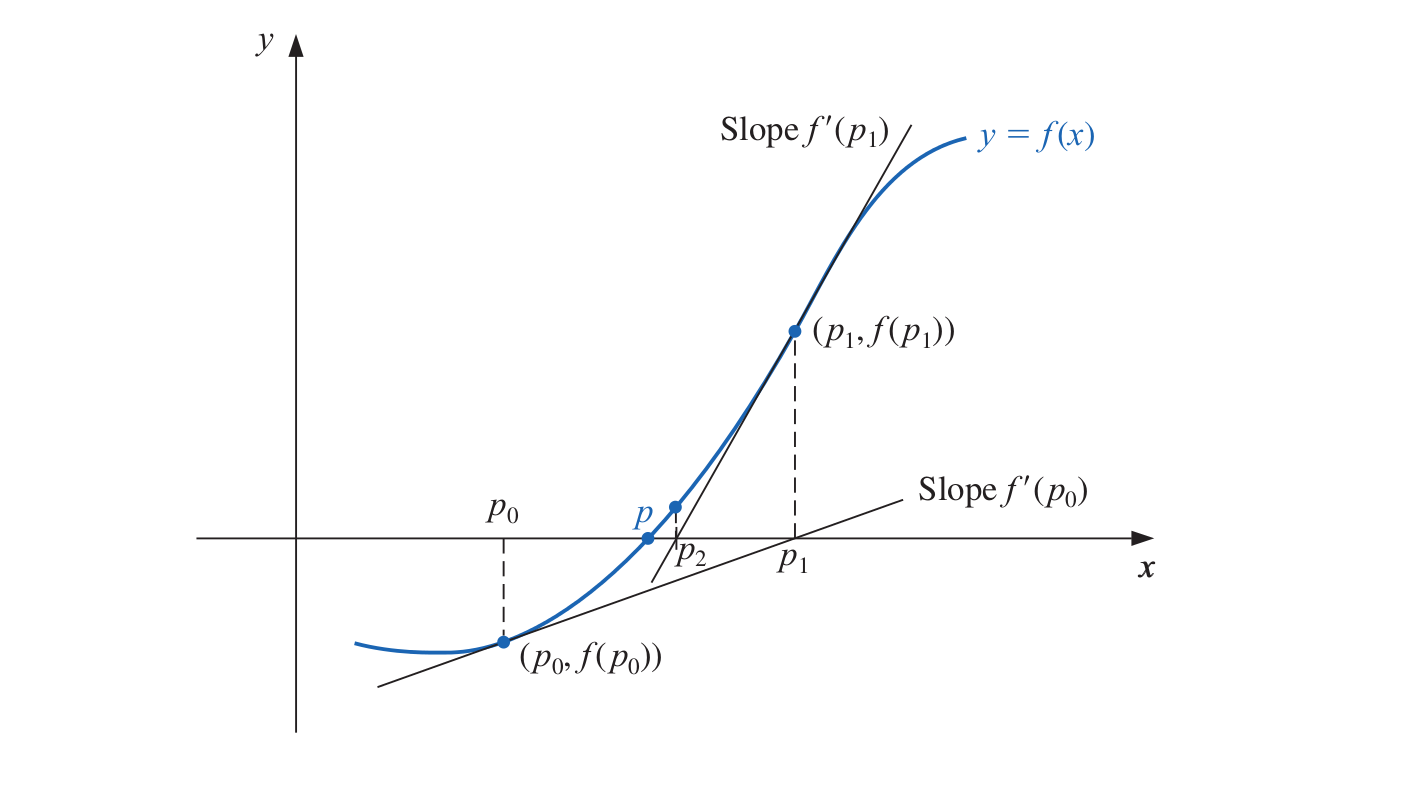
\includegraphics[scale = 0.27]{imagenes/newton.png}~\\[0.25cm]
\end{center}

Sea $\{x_n\}_n$ una iteración de Newton. Dado $x_n$, definimos $x_{n + 1}$ como la abscisa de la intersección entre la recta tangente a $f$ en $x_n$ y el eje $x$. La recta tangente a $f$ en $x_n$ es $y = f'(x_n)x + b$ siendo $b$ la ordenada al origen. Para $x = x_n$, esta recta toma el valor $y = f(x_n)$, con lo cual $f(x_n) = f'(x_n) x_n + b$, i. e., $b = f(x_n) - x_n f'(x_n)$. Luego, la recta tangente a $f$ en $x_n$ es

\[y = f'(x_n)x + f(x_n) - x_n f'(x_n)\]

La intersección entre esta recta y el eje $x$ se da para un valor $x$ tal que $f'(x_n) x + f(x_n) - x_n f'(x_n) = 0$, i. e., $x = x_n - \frac{f(x_n)}{f'(x_{n})}$. Habíamos definido $x_{n + 1}$ como este valor, con lo cual

\[x_{n + 1} = x_n - \frac{f(x_n)}{f'(x_{n})}\]

\subsubsection{Ventajas y desventajas}

\paragraph{Ventajas}
\begin{itemize}
\item Bajo ciertas condiciones, el método converge con velocidad cuadrática, lo que significa que, a nivel práctico, el número de cifras decimales correctas calculadas se duplica a cada paso.
\end{itemize}

\paragraph{Desventajas}
\begin{itemize}
\item La convergencia está asegurada sólo en un entorno del punto fijo buscado. En general, no conocemos dicho punto y mucho menos cuán cerca del mismo debemos comenzar a iterar.

\item La velocidad de convergencia, a nivel práctico, puede resultar lenta lejos del punto fijo. Esto se debe a que, como vimos antes,

\[\frac{e_{n + 1}}{e_n^2} = \frac{1}{2} \frac{f''(\xi_n)}{f'(x_n)}\]

con lo cual, si $|f'(x_n)|$ es chico, el error decrece lento.

\item Es necesario computar $f'(x_n)$ en cada iteracion. En ciertas situaciones esto puede ser caro de computar o directamente imposible. El método de la Secante viene a salvar este problema.
\end{itemize}

\subsection{Método de la Secante}

El método comienza con dos puntos $x_0$ y $x_1$. La iteración $x_{n + 1}$ es igual a la iteración de Newton, excepto que aproximamos $f'(x_n)$ por la pendiente de la recta secante que pasa por $f(x_{n})$ y $f(x_{n - 1})$.

\begin{center}
	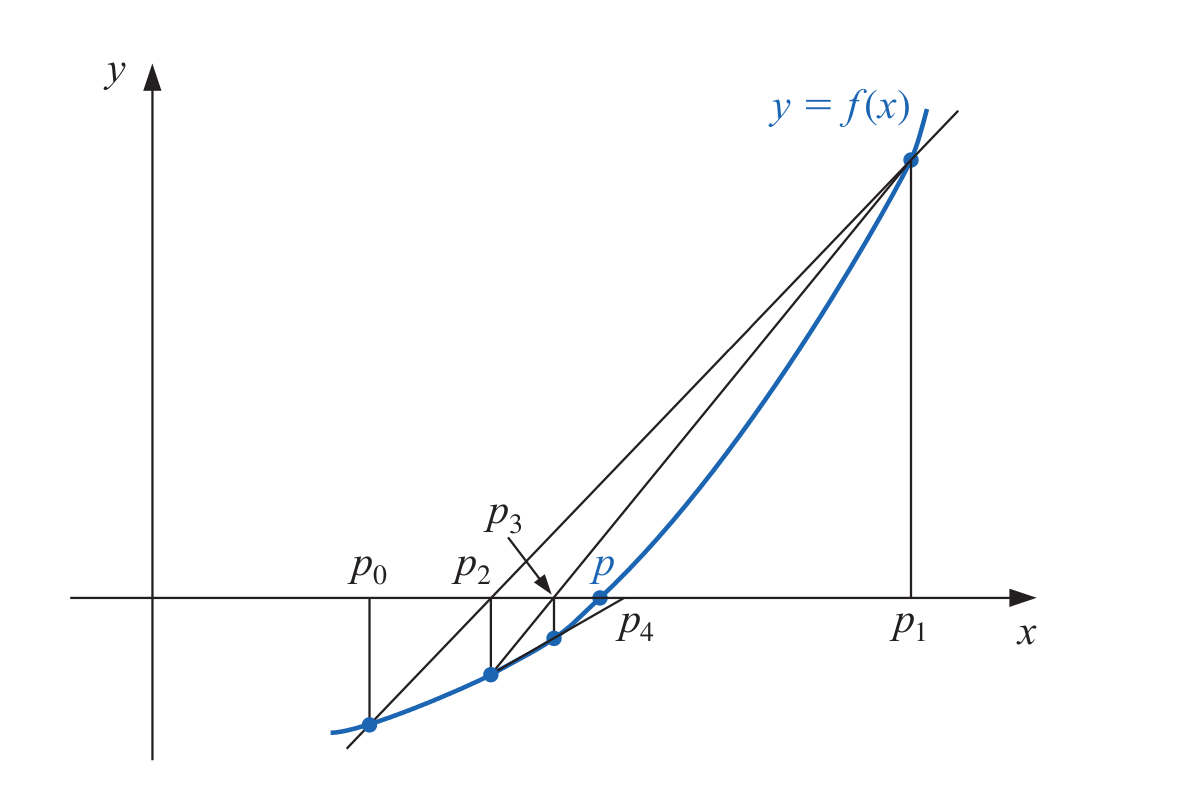
\includegraphics[scale = 0.23]{imagenes/secante.png}~\\[0.25cm]
\end{center}

Explícitamente, la aproximación que estamos usando es

\[f'(x_n) = \frac{f(x_n) - f(x_{n - 1})}{x_n - x_{n - 1}}\]

Por lo tanto, la sucesión que usa este método está dada por

\[x_{n + 1} = x_n - \frac{f(x_n)}{\frac{f(x_n) - f(x_{n - 1})}{x_n - x_{n - 1}}} = x_n - \frac{f(x_n)(x_n - x_{n - 1})}{f(x_n) - f(x_{n - 1})}\]

Se puede demostrar que la velocidad de este método es supralineal.

\subsubsection{Ventajas y desventajas}

\paragraph{Ventajas}
\begin{itemize}
\item No es necesario computar ningún valor de $f'$.
\end{itemize}

\paragraph{Desventajas}
\begin{itemize}
\item La velocidad de convergencia es más lenta que la del método de Newton.

\item A medida que $n$ crece y $x_n$ va convergiendo, $x_n \approx x_{n - 1}$ y $f(x_n) \approx f(x_{n - 1})$, lo que produce una pérdida de dígitos significativos debido al redondeo en el término $\frac{f(x_n)(x_n - x_{n - 1})}{f(x_n) - f(x_{n - 1})}$. El método Regula Falsi provee una solución a este problema.
\end{itemize}

\subsection{Método Regula Falsi}

Genera aproximaciones del mismo modo que el método de la Secante, pero en cada paso verifica que la raíz buscada quede entre dos iteraciones sucesivas, en forma análoga al método de Bisección.

Comienza con dos puntos $x_0$ y $x_1$ tal que $f(x_0)f(x_1) < 0$. Dados $x_{n - 1}$ y $x_n$, el punto $x_{n + 1}$ se calcula mediante la intersección de la recta secante que pasa por $f(x_{n - 1})$ y $f(x_n)$, y el eje $x$. Luego, redefine $x_n$ como aquel valor $x_{n - 1}$ o $x_n$ que tiene distinto signo (evaluado en $f$) que $x_{n + 1}$. La fórmula de la iteración sigue siendo la misma del método de la Secante.

En otras palabras, es idéntico al método de Bisección excepto que, en lugar de quedarse con el punto medio, toma la intersección entre la secante y el eje $x$.

Se puede probar que la velocidad de convergencia del método es al menos $\varphi = \frac{1 + \sqrt{5}}{2}$.

\subsubsection{Ventajas y desventajas}

\paragraph{Ventajas}
\begin{itemize}
\item Desde el punto de vista numérico, ahora $f(x_n)$ y $f(x_{n - 1})$ siempre tendrán distinto signo, con lo cual $f(x_n) - f(x_{n - 1})$ es una resta entre números de distinto signo (podemos pensar que es una suma), evitando una cancelación catastrófica.
\end{itemize}

\paragraph{Desventajas}
\begin{itemize}
\item Requiere más operaciones que el método de la secante.
\end{itemize}